\documentclass{article}

\usepackage{fancyhdr}
\usepackage{extramarks}
\usepackage{amsmath}
\usepackage{amsthm}
\usepackage{amsfonts}
\usepackage{tikz}
\usepackage[plain]{algorithm}
\usepackage{algpseudocode}
\usepackage{xcolor}
\usepackage{enumitem}
\usepackage{amssymb}
\usepackage{todonotes}
\usepackage{mathtools}
\usepackage{wasysym}
\usepackage{cancel}

\usetikzlibrary{automata,positioning}

%
% Basic Document Settings
%

\topmargin=-0.45in
\evensidemargin=0in
\oddsidemargin=0in
\textwidth=6.5in
\textheight=9.0in
\headsep=0.25in

\linespread{1.1}

\pagestyle{fancy}
\lhead{\hmwkAuthorName}
\chead{\hmwkClass\ (\hmwkClassInstructor): \hmwkTitle}
\rhead{\firstxmark}
\lfoot{\lastxmark}
\cfoot{\thepage}

\renewcommand\headrulewidth{0.4pt}
\renewcommand\footrulewidth{0.4pt}

\setlength\parindent{0pt}

%
% Create Problem Sections
%

\newcommand{\enterProblemHeader}[1]{
    \nobreak\extramarks{}{Problem \arabic{#1} continued on next page\ldots}\nobreak{}
    \nobreak\extramarks{Problem \arabic{#1} (continued)}{Problem \arabic{#1} continued on next page\ldots}\nobreak{}
}

\newcommand{\exitProblemHeader}[1]{
    \nobreak\extramarks{Problem \arabic{#1} (continued)}{Problem \arabic{#1} continued on next page\ldots}\nobreak{}
    \stepcounter{#1}
    \nobreak\extramarks{Problem \arabic{#1}}{}\nobreak{}
}

\newcount\colveccount
\newcommand*\colvec[1]{
        \global\colveccount#1
        \begin{pmatrix}
        \colvecnext
}
\def\colvecnext#1{
        #1
        \global\advance\colveccount-1
        \ifnum\colveccount>0
                \\
                \expandafter\colvecnext
        \else
                \end{pmatrix}
        \fi
}

\setcounter{secnumdepth}{0}
\newcounter{partCounter}
\newcounter{homeworkProblemCounter}
\setcounter{homeworkProblemCounter}{1}
\nobreak\extramarks{Problem \arabic{homeworkProblemCounter}}{}\nobreak{}

%
% Homework Problem Environment
%
% This environment takes an optional argument. When given, it will adjust the
% problem counter. This is useful for when the problems given for your
% assignment aren't sequential. See the last 3 problems of this template for an
% example.
%
\newenvironment{homeworkProblem}[1][-1]{
    \ifnum#1>0
        \setcounter{homeworkProblemCounter}{#1}
    \fi
    \section{Problem \arabic{homeworkProblemCounter}}
    \setcounter{partCounter}{1}
    \enterProblemHeader{homeworkProblemCounter}
}{
    \exitProblemHeader{homeworkProblemCounter}
}

%
% Homework Details
%   - Title
%   - Due date
%   - Class
%   - Section/Time
%   - Instructor
%   - Author
%

\newcommand{\hmwkTitle}{Assignment 4}
\newcommand{\hmwkDueDate}{November 15, 2018}
\newcommand{\hmwkClass}{AFL}
\newcommand{\hmwkClassTime}{Fall Semester}
\newcommand{\hmwkClassInstructor}{Prof. Laura Pozzi}
\newcommand{\hmwkAuthorName}{\textbf{A. Romanelli}}

%
% Title Page
%

\title{
    \vspace{2in}
    \textmd{\textbf{\hmwkClass:\ \hmwkTitle}}\\
    \normalsize\vspace{0.1in}\small{Due\ on\ \hmwkDueDate\ at 11:55pm}\\
    \vspace{0.1in}\large{\textit{\hmwkClassInstructor}}
    \vspace{3in}
}

\author{\hmwkAuthorName}
\date{}

\renewcommand{\part}[1]{\textbf{\large Part \Alph{partCounter}}\stepcounter{partCounter}\\}

%
% Various Helper Commands
%

% Useful for algorithms
\newcommand{\alg}[1]{\textsc{\bfseries \footnotesize #1}}

% For derivatives
\newcommand{\deriv}[1]{\frac{\mathrm{d}}{\mathrm{d}x} (#1)}

% For partial derivatives
\newcommand{\pderiv}[2]{\frac{\partial}{\partial #1} (#2)}

% Integral dx
\newcommand{\dx}{\mathrm{d}x}

% Alias for the Solution section header
\newcommand{\solution}{\textbf{\large Solution}}

% Probability commands: Expectation, Variance, Covariance, Bias
\newcommand{\E}{\mathrm{E}}
\newcommand{\Var}{\mathrm{Var}}
\newcommand{\Cov}{\mathrm{Cov}}
\newcommand{\Bias}{\mathrm{Bias}}

\begin{document}

\maketitle

\pagebreak

\begin{homeworkProblem}
	\paragraph{Prove that:} Language $L1 = \{ w | w \text{ has more 0s than 1s}\}$ is not regular. \\ \\
	Let's assume that language $L1$ is a regular language, then there must exist $p$ such that all strings of length $p$ can be pumped.\\\\ We'll choose a $p$ such that the corresponding strings express the non regularity of language $L1$:
	$$s = 1^{p}0^{p+1}$$
	\begin{center}
		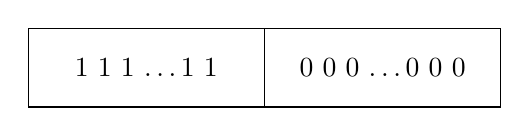
\begin{tikzpicture}
			\draw (0,0) rectangle (3,1);
			\node at (1.5,0.5) {1 1 1 \dots 1 1};
			\draw (3,0) rectangle (6,1);
			\node at (4.5,0.5) {0 0 0 \dots 0 0 0};
		\end{tikzpicture}
	\end{center}
	We need to obey the three following conditions:
	\begin{enumerate}
		\item $xy^iz \in L1, \forall i \geq 0$,
		\item $|y| > 0$,
		\item $|xy| \leq p$
	\end{enumerate}
	The third condition imposes that our $y$ must consist of only 1s. \\
	The second condition imposes that our $y$ consists of at least one symbol.
	The first condition can now be no longer satisfied, as repeating the ones $i$ times will cause the string to no longer belong to $L1$, since it will have more 1s than 0s.
	
\end{homeworkProblem}
\begin{homeworkProblem}
	\paragraph{Prove that:} Language $L2 = \{ w | w \text{ has even length and the first half of w has more 0s than the second half of w}\}$\\ \\
	We repeat the same process picking a string $s$ which represents the non regularity of $L2$ and that can't possibly be pumped:
	$$s = 1^p0^p1^{2p}$$
		\begin{center}
		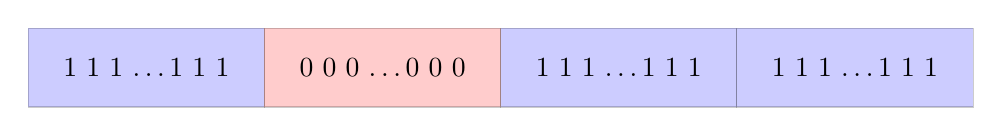
\begin{tikzpicture}
			\fill[fill=blue, opacity=0.2, draw=black] (0,0) rectangle (3,1);
			\node at (1.5,0.5) {1 1 1 \dots 1 1 1};
			\draw[fill=red, opacity=0.2, draw=black] (3,0) rectangle (6,1);
			\node at (4.5,0.5) {0 0 0 \dots 0 0 0};
			\filldraw[fill=blue, opacity=0.2, draw=black] (6,0) rectangle (9,1);
			\node at (7.5,0.5) {1 1 1 \dots 1 1 1};
			\filldraw[fill=blue, opacity=0.2, draw=black] (9,0) rectangle (12,1);
			\node at (10.5,0.5) {1 1 1 \dots 1 1 1};
		\end{tikzpicture}
	\end{center}
	Because of the third condition, we know that $y$ will be made up exclusively by 1s. \\
	The second condition also reassures us that $y$ must consist of at least a symbol. \\
	To formally demonstrate how $xy^iz \notin L2$ we can imagine a very large $i$ and $|y|$ as well. \\
	 Let $|y|$ be at its maximum, the closest to the condition $|xy| \leq p$ as possible, so that $y = 1^p$. \\ 
	 Now, pumping this string with $i \geq 1$ will result in the string of form:
	 $$s' = 1^i0^p1^{2p}$$
	 $$ x = \epsilon, y = 1^i, z = 0^p1^2p$$ 
	 It's clearly visible that the first condition falls apart with $i \geq 2$, since it will result in an equal amount of zeros on both left and right side. \\
	 If instead of $y = 1^p$ we had picked $y = 1$ the result would be no different, $i$ would simply need to be $i \geq 2p$ in order to achieve the same result. Hence we can definitely conclude that exists some $i \in \mathbb{N} | xy^iz \notin L2$, as we have already seen.
\end{homeworkProblem}

\end{document}
